%%
%% This is file `sigconf.tex',
%% generated with the docstrip utility.
%%
%% The original source files were:
%%
%% samples.dtx  (with options: `all,proceedings,sigconf')
%% 
%% IMPORTANT NOTICE:
%% 
%% For the copyright see the source file.
%% 
%% Any modified versions of this file must be renamed
%% with new filenames distinct from sigconf.tex.
%% 
%% For distribution of the original source see the terms
%% for copying and modification in the file samples.dtx.
%% 
%% This generated file may be distributed as long as the
%% original source files, as listed above, are part of the
%% same distribution. (The sources need not necessarily be
%% in the same archive or directory.)
%%
%%
%% Commands for TeXCount
%TC:macro \cite [option:text,text]
%TC:macro \citep [option:text,text]
%TC:macro \citet [option:text,text]
%TC:envir table 0 1
%TC:envir table* 0 1
%TC:envir tabular [ignore] word
%TC:envir displaymath 0 word
%TC:envir math 0 word
%TC:envir comment 0 0
%%
%% The first command in your LaTeX source must be the \documentclass
%% command.
%%
%% For submission and review of your manuscript please change the
%% command to \documentclass[manuscript, screen, review]{acmart}.
%%
%% When submitting camera ready or to TAPS, please change the command
%% to \documentclass[sigconf]{acmart} or whichever template is required
%% for your publication.
%%
%%
\documentclass[sigconf]{acmart}
%%
%% \BibTeX command to typeset BibTeX logo in the docs
\AtBeginDocument{%
  \providecommand\BibTeX{{%
    Bib\TeX}}}

\usepackage[T1]{fontenc}
\usepackage[utf8]{inputenc}
\usepackage{lmodern}
\usepackage{microtype}
\usepackage{amsmath,amssymb}
\usepackage{booktabs,tabularx,array}
\usepackage{xcolor}
\usepackage{enumitem}
\usepackage{caption}
\usepackage{needspace}
\usepackage{fancyvrb}
\usepackage[round,authoryear]{natbib}

\definecolor{draftred}{RGB}{145,38,45}
\newcommand{\placeholder}[1]{\textcolor{draftred}{\textbf{[\,\textit{#1}\,]}}}
\newcommand{\draftnote}[1]{%
  \par\smallskip\noindent{\small\color{draftred}\textbf{Draft note.} #1}\par\smallskip}
\newcommand{\TBD}{\textcolor{draftred}{TBD}}
\newcommand{\NA}{\textemdash}
\newcommand{\ind}{\mathbb{I}}
%% Rights management information.  This information is sent to you
%% when you complete the rights form.  These commands have SAMPLE
%% values in them; it is your responsibility as an author to replace
%% the commands and values with those provided to you when you
%% complete the rights form.
\setcopyright{acmlicensed}
\copyrightyear{2018}
\acmYear{2018}
\acmDOI{XXXXXXX.XXXXXXX}
%% These commands are for a PROCEEDINGS abstract or paper.
\acmConference[Conference acronym 'XX]{Make sure to enter the correct
  conference title from your rights confirmation email}{June 03--05,
  2018}{Woodstock, NY}
%%
%%  Uncomment \acmBooktitle if the title of the proceedings is different
%%  from ``Proceedings of ...''!
%%
%%\acmBooktitle{Woodstock '18: ACM Symposium on Neural Gaze Detection,
%%  June 03--05, 2018, Woodstock, NY}
\acmISBN{978-1-4503-XXXX-X/2018/06}


%%
%% Submission ID.
%% Use this when submitting an article to a sponsored event. You'll
%% receive a unique submission ID from the organizers
%% of the event, and this ID should be used as the parameter to this command.
%%\acmSubmissionID{123-A56-BU3}

%%
%% For managing citations, it is recommended to use bibliography
%% files in BibTeX format.
%%
%% You can then either use BibTeX with the ACM-Reference-Format style,
%% or BibLaTeX with the acmnumeric or acmauthoryear sytles, that include
%% support for advanced citation of software artefact from the
%% biblatex-software package, also separately available on CTAN.
%%
%% Look at the sample-*-biblatex.tex files for templates showcasing
%% the biblatex styles.
%%
%%
%% The majority of ACM publications use numbered citations and
%% references.  The command \citestyle{authoryear} switches to the
%% "author year" style.
%%
%% If you are preparing content for an event
%% sponsored by ACM SIGGRAPH, you must use the "author year" style of
%% citations and references.
%% Uncommenting
%% the next command will enable that style.
%%\citestyle{acmauthoryear}


%%
%% end of the preamble, start of the body of the document source.
\begin{document}

%%
%% The "title" command has an optional parameter,
%% allowing the author to define a "short title" to be used in page headers.
\title{Reading Colonial Descriptions of Women at Scale: A Historian-Guided Computational Study of Caribbean Newspapers}

%%
%% The "author" command and its associated commands are used to define
%% the authors and their affiliations.
%% Of note is the shared affiliation of the first two authors, and the
%% "authornote" and "authornotemark" commands
%% used to denote shared contribution to the research.
% \author{Ben Trovato}
% \authornote{Both authors contributed equally to this research.}
% \email{trovato@corporation.com}
% \orcid{1234-5678-9012}
% \author{G.K.M. Tobin}
% \correspondingauthor
% \authornotemark[1]
% \email{webmaster@marysville-ohio.com}
% \affiliation{%
%   \institution{Institute for Clarity in Documentation}
%   \city{Dublin}
%   \state{Ohio}
%   \country{USA}
% }

% \author{Lars Th{\o}rv{\"a}ld}
% \affiliation{%
%   \institution{The Th{\o}rv{\"a}ld Group}
%   \city{Hekla}
%   \country{Iceland}}
% \email{larst@affiliation.org}

% \author{Valerie B\'eranger}
% \affiliation{%
%   \institution{Inria Paris-Rocquencourt}
%   \city{Rocquencourt}
%   \country{France}
% }

% \author{Aparna Patel}
% \affiliation{%
%  \institution{Rajiv Gandhi University}
%  \city{Doimukh}
%  \state{Arunachal Pradesh}
%  \country{India}}

% \author{Huifen Chan}
% \affiliation{%
%   \institution{Tsinghua University}
%   \city{Haidian Qu}
%   \state{Beijing Shi}
%   \country{China}}

% \author{Charles Palmer}
% \affiliation{%
%   \institution{Palmer Research Laboratories}
%   \city{San Antonio}
%   \state{Texas}
%   \country{USA}}
% \email{cpalmer@prl.com}

% \author{John Smith}
% \affiliation{%
%   \institution{The Th{\o}rv{\"a}ld Group}
%   \city{Hekla}
%   \country{Iceland}}
% \email{jsmith@affiliation.org}

% \author{Julius P. Kumquat}
% \correspondingauthor
% \affiliation{%
%   \institution{The Kumquat Consortium}
%   \city{New York}
%   \country{USA}}
% \email{jpkumquat@consortium.net}

%%
%% By default, the full list of authors will be used in the page
%% headers. Often, this list is too long, and will overlap
%% other information printed in the page headers. This command allows
%% the author to define a more concise list
%% of authors' names for this purpose.
\renewcommand{\shortauthors}{Trovato et al.}

%%
%% The abstract is a short summary of the work to be presented in the
%% article.
\begin{abstract}
Digitized Caribbean newspapers preserve the language through which colonial print represented women in relation to gender, racialization, labor, and social status. Recovering these descriptions is difficult because historical spelling variation and optical character recognition (OCR) errors obstruct retrieval, while computational interpretation risks turning source classifications into unqualified claims about the people described. We present a historian-guided framework for studying representations of enslaved, indentured, and free women in Danish newspapers. 



It explicitly separates source wording, structured annotation, and historical inference, and preserves uncertainty where the evidence does not support a determinate conclusion. We evaluate women-description retrieval and person/labor description answering against Gemini-authored reference VQA items and controlled comparisons with off-the-shelf vision--language models, OCR pipelines, and a LoRA/RL-adapted Qwen3-VL system. On the Dutch women-related evaluation subset ($n{=}24$), the adapted model reaches mean token F1 $0.479$ versus $0.251$ for base Qwen3-VL-2B and $0.075$ for LLaVA-1.5-7B; a proxy audit of automatic women-clip evidence yields only $6/19$ keyword-supported snippets ($\approx 0.32$ precision), underscoring retrieval noise. By connecting aggregate reliability estimates to traceable archival passages, the study offers an evaluated approach to examining colonial representations without treating them as transparent accounts of women's identities or experiences. Its contribution is not the reconstruction of voices absent from the record, but a reproducible account of what the surviving evidence supports and how computational mediation changes its interpretation.

\end{abstract}

%%
%% The code below is generated by the tool at http://dl.acm.org/ccs.cfm.
%% Please copy and paste the code instead of the example below.
%%
\begin{CCSXML}
<ccs2012>
 <concept>
  <concept_id>00000000.0000000.0000000</concept_id>
  <concept_desc>Do Not Use This Code, Generate the Correct Terms for Your Paper</concept_desc>
  <concept_significance>500</concept_significance>
 </concept>
 <concept>
  <concept_id>00000000.00000000.00000000</concept_id>
  <concept_desc>Do Not Use This Code, Generate the Correct Terms for Your Paper</concept_desc>
  <concept_significance>300</concept_significance>
 </concept>
 <concept>
  <concept_id>00000000.00000000.00000000</concept_id>
  <concept_desc>Do Not Use This Code, Generate the Correct Terms for Your Paper</concept_desc>
  <concept_significance>100</concept_significance>
 </concept>
 <concept>
  <concept_id>00000000.00000000.00000000</concept_id>
  <concept_desc>Do Not Use This Code, Generate the Correct Terms for Your Paper</concept_desc>
  <concept_significance>100</concept_significance>
 </concept>
</ccs2012>
\end{CCSXML}

\ccsdesc[500]{Do Not Use This Code~Generate the Correct Terms for Your Paper}
\ccsdesc[300]{Do Not Use This Code~Generate the Correct Terms for Your Paper}
\ccsdesc{Do Not Use This Code~Generate the Correct Terms for Your Paper}
\ccsdesc[100]{Do Not Use This Code~Generate the Correct Terms for Your Paper}

%%
%% Keywords. The author(s) should pick words that accurately describe
%% the work being presented. Separate the keywords with commas.
\keywords{historical newspapers, colonial archives, women and slavery, visual question answering, OCR, Cura\c{c}ao, digital humanities}
%% A "teaser" image appears between the author and affiliation
%% information and the body of the document, and typically spans the
%% page.
% \begin{teaserfigure}
%  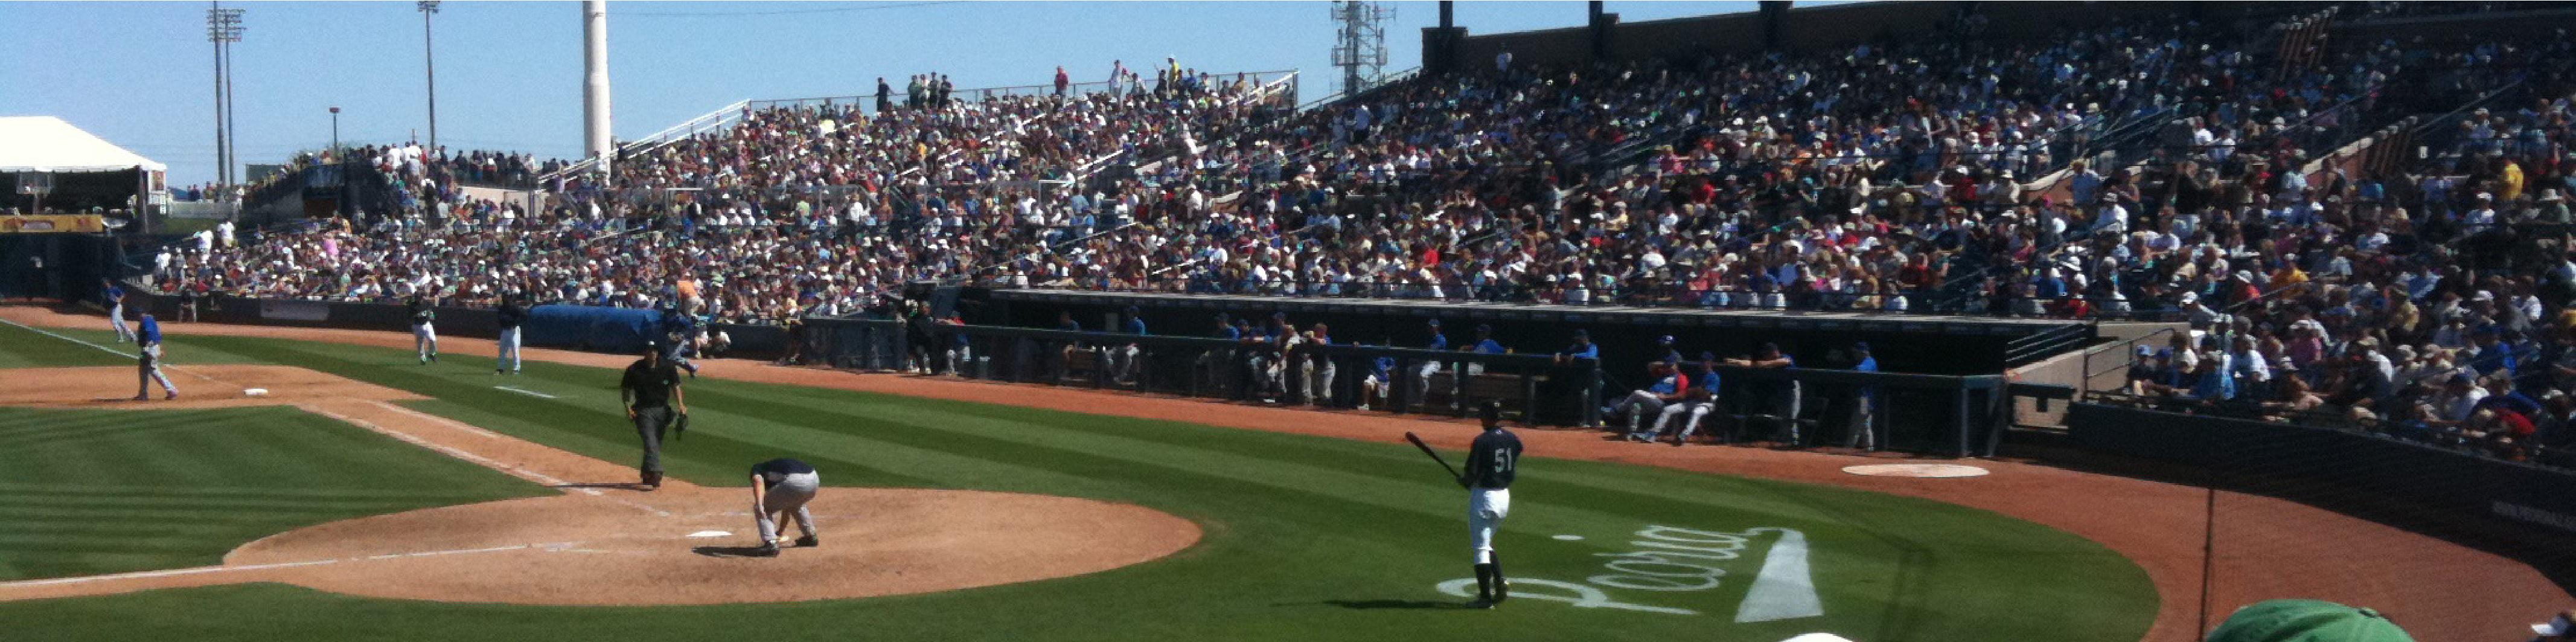
\includegraphics[width=\textwidth]{sampleteaser}
%   \caption{Seattle Mariners at Spring Training, 2010.}
%   \Description{Enjoying the baseball game from the third-base
%   seats. Ichiro Suzuki preparing to bat.}
%   \label{fig:teaser}
% \end{teaserfigure}

\received{20 February 2007}
\received[revised]{12 March 2009}
\received[accepted]{5 June 2009}

%%
%% This command processes the author and affiliation and title
%% information and builds the first part of the formatted document.
\maketitle

% ======================================================================
\section{Introduction}
\label{sec:introduction}
% ======================================================================

Recovering a description of a woman from a colonial newspaper is not the same as recovering her perspective. A passage may make her visible through a transaction, an allegation, a labor relationship, or an institutional encounter while revealing little about how she understood her own circumstances. Scholarship on slavery's archives has made the conditions of such visibility central to historical interpretation, emphasizing both the possibilities and the limits of working with records produced through unequal power relations \citep{hartman2008venus,fuentes2016dispossessed}. For computational analysis, this distinction must become an operational requirement rather than remain only an interpretive caution.

The present study examines the language used to describe enslaved, indentured, and free women in digitized Caribbean newspapers. Its historical question concerns how descriptive vocabularies and relational frames vary across time, place, and legal or labor arrangements. Its methodological question concerns how these patterns can be measured without confusing what a newspaper asserts with what the historical evidence establishes. A system that correctly retrieves a passage but restates its accusation as fact may be technically useful and historically misleading at the same time.

Two challenges therefore need to be addressed together. \textbf{First}, spelling variation, damaged scans, and OCR errors can prevent relevant descriptions from being retrieved or interpreted. Research on historical newspapers has demonstrated the potential of LLM-based post-OCR correction \citep{thomas2024leveraging}. However, correction itself requires scrutiny: a separate study of eighteenth-century Russian print identifies historically inappropriate character insertions and reports that post-correction can reduce accuracy in that setting \citep{levchenko2025evaluating}. These findings motivate evaluating historical fidelity rather than assuming that more readable text is necessarily more faithful text. \textbf{Second}, the language being recovered is itself an object of historical analysis. A model must preserve evidence of colonial framing without adopting that framing as its own account. This requires explicit source attribution, a distinction between quotation and interpretation, and a way to withhold conclusions when a passage is ambiguous. We treat these requirements as measurable properties of an analytical system, not as consequences automatically guaranteed by fluent output or a generic instruction to behave like a historian.

We propose a historian-guided framework in which domain expertise informs retrieval vocabularies, extraction categories, prompt examples, reference annotations, and the interpretation of aggregate patterns. Each extracted claim remains linked to its supporting passage. Legal status, labor arrangements, racialized descriptions, and represented agency are recorded as distinct dimensions rather than collapsed into a single classification. The analysis combines longitudinal measurement with close reading, and evaluates automated outputs separately from records corrected through human review.

The study addresses three research questions:
\begin{itemize}
  \item \textbf{RQ1: Historical change.} How do descriptions of women vary across periods, territories, newspaper genres, and documented legal or labor arrangements?
  \item \textbf{RQ2: Analytical reliability.} How reliably can a historian-guided framework retrieve and interpret these descriptions under OCR degradation and historical ambiguity?
  \item \textbf{RQ3: Model-mediated distortion.} When do foundation models convert source perspectives into unsupported claims, and which forms of historian guidance reduce these errors?
\end{itemize}

The intended contributions are a historically situated analysis of changing representations, an evidence-grounded computational framework, and a controlled evaluation of extraction and interpretive reliability. Together, they connect the scale of computational analysis to the accountability of source-based historical argument. We do not equate the number of recovered mentions with the number of distinct women, or treat greater textual visibility as evidence of greater social autonomy.

% ======================================================================
\section{Historical Context and Related Work}
\label{sec:related}
% ======================================================================

\subsection{Women, Colonial Print, and the Archive}

Our interpretive starting point is that archival descriptions require analysis of the circumstances under which they were produced. Hartman's discussion of the archive of Atlantic slavery foregrounds the limits of knowledge about enslaved women and the conditions that shape their appearance in the record \citep{hartman2008venus}. Fuentes's study of eighteenth-century Bridgetown similarly examines how colonial power and archival production constrain what can be known from fragmentary accounts of women \citep{fuentes2016dispossessed}. These works inform our distinction between making a passage computationally accessible and claiming to have recovered an unmediated historical voice.

The empirical core of this paper is Dutch colonial print from \textbf{Cura\c{c}ao}, centered on \textit{De Cura\c{c}aosche courant}. The newspaper's notices, advertisements, shipping lists, and official proclamations are a primary medium through which women appear as named persons, unnamed \textit{vrouwspersonen}, widows managing print shops or estates, or racialized and status-marked bodies in legal and commercial prose. Dutch Caribbean emancipation (1~July~1863) supplies the principal legal watershed for periodization: our digitized pages fall overwhelmingly in the late-slavery decades (1816--1862). We therefore treat ``post-emancipation'' comparisons as out of scope until the corpus is extended past 1863. Indenture after abolition is likewise not attested in the present sample and is retained in the schema only as a reserved category for future issues.
\draftnote{Expand with territory-specific historiography (free Black and colored women in Willemstad; manumission; Sephardic and Protestant print networks; Venezuelan/Caribbean news circuits) and add supporting references beyond Hartman/Fuentes.}

For this study, status categories are analytical variables with documented meanings, not timeless descriptions. We distinguish terminology appearing in a source from categories assigned by the research team. We also distinguish formal legal classification, stated labor arrangements, and the broader constraints that historians identify through contextual interpretation. The schema retains unknown and disputed values rather than resolving them through assumptions about names, occupations, or racialized language.

\subsection{Historical Text Processing and Semantic Change}

Thomas et al.\ demonstrate prompt-based, instruction-tuned post-OCR correction for nineteenth-century British newspapers \citep{thomas2024leveraging}. Levchenko's evaluation of historical-document OCR highlights the need to test preservation of period-specific textual features as well as conventional transcription accuracy \citep{levchenko2025evaluating}. Our methodological focus is the relationship between preprocessing and downstream historical claims: a change that improves retrieval may still alter the very descriptors under investigation.

Distributional approaches provide methods for examining lexical meaning over time. Hamilton et al.\ develop diachronic word-embedding analyses \citep{hamilton2016diachronic}, while Dubossarsky et al.\ show that some apparent regularities of semantic change can reflect properties of the representations and word frequency rather than historical change alone \citep{dubossarsky2017outta}. Accordingly, we distinguish lexical prevalence, contextual semantic variation, and changes in relational framing. Quantitative displacement is treated as a candidate signal for interpretation, not a historical conclusion by itself.

\subsection{Expert Annotation and Model-Output Auditing}

We define model-mediated distortion in relation to specific analytical failures. This follows the need, articulated by Blodgett et al., to make the normative assumptions and target behaviors of bias evaluation explicit \citep{blodgett2020language}. The source may contain dehumanizing language without an accurate quotation of that language constituting model endorsement. Conversely, an apparently neutral summary may distort the evidence by removing an allegation's source or suppressing explicit coercion.

Expert annotation also requires a treatment of disagreement. Work on subjective annotation shows why aggregation into a single majority label can discard meaningful variation \citep{davani2022dealing}. We therefore distinguish transcription disputes, disagreements about applying the schema, and defensible interpretive differences. Historian-adjudicated reference annotations support evaluation, but do not constitute an exhaustive or interpretation-free account of the past.

% ======================================================================
\section{Corpus and Research Design}
\label{sec:corpus}
% ======================================================================

\subsection{Sources, Coverage, and Provenance}

The corpus comprises \textbf{one primary newspaper title}---\textit{De Cura\c{c}aosche courant}---from digitized Cura\c{c}ao holdings used in this project (sample original PDFs plus page images), covering the Dutch Caribbean territory of \textbf{Cura\c{c}ao}, language \textbf{Dutch} (historical orthography), and dates \textbf{1816--1862}. Inclusion criteria are pages/issues that (i)~are readable enough for visual QA or clip extraction and (ii)~belong to the curated Racialized Motherhood / Dutch VQA digitization set. Excluded material comprises non-Cura\c{c}ao titles held elsewhere in the repository (e.g.\ \textit{The Quebec Gazette}, Spanish \textit{Revista econ\'{o}mica}), which support multilingual VQA diagnostics but are \emph{not} used for the women-description claims in this paper. Table~\ref{tab:corpus} records the information needed to define the study's empirical scope.

\begin{table}[tbp]
\centering
\caption{Corpus documentation for the Cura\c{c}ao women-description study. Counts refer to currently digitized project files, not the full historical print run.}
\label{tab:corpus}
\small
\begin{tabularx}{\linewidth}{@{}p{0.29\linewidth}Y@{}}
\toprule
\textbf{Field} & \textbf{Required information} \\
\midrule
Collections and access & Project digitizations of \textit{De Cura\c{c}aosche courant}; sample original PDFs under \texttt{Racialized\_Motherhood/}; page JPEGs under \texttt{data/Dutch/extracted\_images of Dutch}. Reuse subject to archive/provider terms (see Data Availability). \\
Titles and territories & \textit{De Cura\c{c}aosche courant}; Willemstad / Cura\c{c}ao and subordinate islands as named in mastheads and proclamations. \\
Dates and languages & Sample PDFs: 1816, 1826, 1836, 1846, 1856. Page-image set: 1819--1862. Language: Dutch (period spelling). Coverage is sparse and issue-selected, not a continuous run. \\
Digitized extent & 5 sample PDFs; 55 page images in the Dutch image directory; 21 pages processed by the women-clip detector; 200 Gemini VQA items (20 pages $\times$ 10 categories). \\
Retrieved material & 36 automatic women-region detections (clips); 19 detections with non-empty evidence strings; 24 women-related VQA items (all 20 PD items plus keyword matches). \\
Quality and repetition & Clip detector shows substantial false positives (proxy evidence precision $\approx 0.32$). Duplicate/near-duplicate clip boxes observed on some pages. OCR quality varies; unreadable spans retained as uncertain. \\
Reference annotations & Gemini-authored VQA gold for TE/NE/TI/MQ/OL/PD/LE/AT/LD/HR. Historian preference pack prepared ($n{=}200$ pairs) but preferences not yet completed. No full independent historian gold for span-level women mentions yet. \\
\bottomrule
\end{tabularx}
\end{table}

The proposed inventory preserves document and page identifiers, issue dates, newspaper titles, and links to page images where available. Publication location is not automatically treated as the location of a reported event. Coverage is summarized by title and time interval so that changes in archival availability can be distinguished from changes in representation. Repeated advertisements and reprints are assigned duplicate-cluster identifiers where detection is sufficiently reliable; analyses with all occurrences and with deduplicated text answer different questions and are reported separately.

\subsection{Periodization and Analytical Categories}

Historical periods for Cura\c{c}ao are defined relative to Dutch Caribbean emancipation on \textbf{1~July~1863}. The present sample is treated as a single \emph{late-slavery} window (1816--1862). Decade bins (1810s--1860s) are used only descriptively for inventory; they are not interpreted as causal period effects without denser coverage. Post-emancipation and post-colonial comparisons are deferred until digitized issues after 1863 are included. Date-based comparisons therefore describe associations within pre-emancipation print, not emancipation effects.

The extraction scheme separates legal status from labor arrangement. In particular, indentured labor is not encoded as a mutually exclusive alternative to every category of legal freedom. Source-explicit labels, contextual interpretations, and uncertainty are recorded separately. The study includes references to girls, unnamed groups (\textit{vrouwen}, \textit{vrouwspersonen}), widows, and people described through racialized or status-marked gendered terms when the source makes the gendered reference explicit; uncertain gendered terms are retained as \emph{uncertain} rather than forced into a binary. All analysis concerns representation in the source, not an automatic determination of personal identity.

\subsection{Units of Analysis and Sampling}

The primary unit is a \emph{contextualized mention}: a reference to a woman or group, its descriptive expressions and relations, and the passage needed to interpret them. A mention is not a unique individual. Cross-document identification requires a separate, validated entity-resolution procedure and is not assumed here.

We propose two complementary evaluation samples. A probability sample of eligible pages or documents is annotated for all relevant mentions, including material not retrieved by the pipeline, to estimate missed evidence. A stratified diagnostic sample provides additional coverage of difficult OCR, rare categories, ambiguous passages, and varied genres. Aggregate estimates use the appropriate sampling weights where needed; the diagnostic sample is not treated as a representative estimate of corpus-wide prevalence. Development material and held-out evaluation material are separated before prompt refinement.

% ======================================================================
\section{Historian-Guided Analytical Framework}
\label{sec:framework}
% ======================================================================

\draftnote{The procedures below form a proposed operational design. Retain only implemented components and replace the remaining choices with the actual software, thresholds, prompts, and review protocol.}

The framework connects five operations: evidence-preserving preprocessing, OCR-aware retrieval, structured extraction, expert validation, and diachronic interpretation. Its organizing principle is a separation between \emph{source wording}, \emph{structured annotation}, and \emph{historical inference}. The first records what is visible in the document, the second assigns explicitly defined analytical fields, and the third develops a contextual argument from the evidence. A plausible inference is never substituted silently for missing source text.

\subsection{OCR-Aware Retrieval and Evidence Preservation}

Each document retains an immutable original OCR layer. Proposed corrections and retrieval-oriented normalization are stored separately, with their provenance and links to the original passage. Modernized spellings may support candidate retrieval, but they are not counted as historical source forms. Unreadable characters remain marked as uncertain unless verified against the image; model-generated completion is not treated as transcription.

Candidate retrieval combines (i)~a historically informed Dutch lexicon of women-related terms (\textit{vrouw}, \textit{vrouwen}, \textit{weduwe}/\textit{wed.}, \textit{meisje}, \textit{moeder}, \textit{slavin}, \textit{juffrouw}, etc.; see \texttt{HISTORICAL\_DUTCH\_WOMEN\_TERMS} in the clip extractor) with (ii)~a vision--language detector (Qwen3-VL) that proposes page regions whose evidence strings describe women or women-related notices. The search vocabulary therefore includes documented period variants and contextual expressions for marriage, birth, death, advertisement, and personal notices. Candidate passages retain surrounding context so that a descriptor is not detached from a negation, quotation, relationship, or attribution. Retrieval thresholds (minimum detector score $0.30$ in the current clip script), context-window expansion, and revision history are recorded in the clip report. Recall is estimated from independently listed pages rather than only from material the detector already selected; the present proxy audit shows many high-confidence boxes whose evidence does not actually mention women.

\subsection{Evidence-Linked Extraction Schema}

For a document $d_i$, the extractor returns a set of records rather than a single summary. Each record contains the fields in Table~\ref{tab:schema}. A document may contain several mentions, and a mention may have several descriptors or relations. Unknown, conflicting, and not-applicable values are kept distinct.

\begin{table}[tbp]
\centering
\caption{Proposed record schema. Source evidence and researcher interpretation are separate fields; actual category definitions require historian review.}
\label{tab:schema}
\small
\begin{tabularx}{\linewidth}{@{}p{0.23\linewidth}Y@{}}
\toprule
\textbf{Field} & \textbf{Content and evidentiary rule} \\
\midrule
Provenance & Document, page, date, text version, and original character offsets \\
Mention & Exact reference to a woman or group; no unvalidated identity linkage \\
Descriptor & Exact expression, context, and separately stored normalized form \\
Status dimensions & Legal status and labor arrangement, each with evidence and uncertainty \\
Attributed relation & Relation, participants, direction, assertion source, and supporting spans \\
Source perspective & Editorial narration, advertisement, quotation, reported institutional statement, or unknown \\
Interpretation & Analytical frame and explanation, distinct from source assertions \\
Review state & Automated, reviewed unchanged, corrected, unresolved, or unreadable \\
\bottomrule
\end{tabularx}
\end{table}

Prompts require evidence spans for extractive assertions and attribution for descriptions supplied by a speaker, advertiser, or institution. They prohibit inferring legal status or racial identity from a name alone. An allegation is recorded as an attributed allegation rather than a verified behavior. Where an interpretation requires context beyond the passage, the additional source is identified; unsupported elaboration is excluded from the extracted record.

\subsection{Historian Guidance and Quality Control}

Historians contribute through a versioned codebook, historically situated examples, ambiguity rules, and an adjudication protocol. Prompt examples are drawn only from development material. Before held-out evaluation, the schema, prompt variants, category mappings, and decision thresholds are fixed. Test outputs do not become new prompt examples during the reported evaluation.

Automated checks verify valid output structure, document identifiers, and whether quoted strings match the specified text version. A matching string establishes traceability, not correctness of interpretation. Human review therefore examines disputed status assignments, attribution, historically consequential corrections, and a random sample of apparently valid records. A review queue based only on model-expressed confidence is insufficient because unnoticed confident errors would remain invisible. The implemented routing policy in the current codebase prepares a historian preference pack of $200$ pairwise answer comparisons (orthographic authenticity and contextual factuality) for Dutch VQA items; preferences are not yet filled, so reported scores below use Gemini reference answers rather than completed historian adjudication. For clip review, we flag empty evidence, empty labels, and evidence strings that fail a women-keyword check as high-priority false-positive candidates.

Review changes are logged separately from initial model outputs. We report the automated system and the human-corrected workflow as different evaluation conditions. Claims about historian guidance refer to the intervention actually used---for example, schema design or prompt examples---rather than implying parameter fine-tuning when no model weights were updated.

\subsection{Diachronic Measurement}

The analysis distinguishes changing prevalence from changing contextual meaning. Let $\mathcal{M}_{t,h}$ denote the included mentions in time interval $t$ and comparison stratum $h$, where $h$ may specify territory, newspaper, and genre. For an analytical frame $c$, a proposed descriptive measure is
\begin{equation}
\widehat{p}_{c,t,h}
=
\frac{\sum_{m\in\mathcal{M}_{t,h}} w_m\,\ind\{c\in C_m\}}
     {\sum_{m\in\mathcal{M}_{t,h}} w_m},
\label{eq:prevalence}
\end{equation}
where $C_m$ is the set of assigned frames and $w_m$ is a sampling weight, or $1$ for a census of the included mentions. Categories may co-occur, so their proportions need not sum to one. Empty cells are reported as unavailable, not zero. The denominator and the treatment of uncertain annotations are stated for every comparison.

Equation~\eqref{eq:prevalence} describes the included corpus; it does not correct unknown retrieval failures or missing archives. To examine corpus-composition effects, we compare estimates within stable strata and, where supported, standardize to common weights over strata observed in the compared periods. Newspaper and genre changes are assessed before attributing a temporal pattern to historical transformation.

Contextual semantic tracking is \emph{not yet implemented} for the Cura\c{c}ao women sample; the present paper reports retrieval and description-answering reliability rather than embedding drift. Planned follow-up uses a shared multilingual encoder with frequency-matched and time-label permutation controls \citep{dubossarsky2017outta}, but those analyses are withheld until denser, cleaner mention sets are available.

\subsection{Intersectional Analysis and Interpretive Audit}

The intersectional analysis examines combinations of source-recorded legal status, labor arrangement, racialized description, and other historically justified dimensions. It does not infer a person's identity from absent evidence or assume that analytical categories are interchangeable across territories. Sparse combinations are reported with their counts and uncertainty rather than converted into rankings of groups.

The model-output audit asks whether the system retains the relationship between a claim and its source. We distinguish unsupported status assignment, loss of attribution, erasure of explicit coercion, unsupported attribution of agency, and unwarranted certainty. These are proposed categories requiring a codebook and expert examples. They should not be combined into a single bias score without a justified weighting rule. Errors in identifying a frame and errors in presenting a source assertion as fact remain analytically distinct.

% ======================================================================
\section{Evaluation: Reliability and Model-Mediated Distortion}
\label{sec:evaluation}
% ======================================================================

\subsection{Reference Annotations and Experimental Setup}

The current benchmark contains \textbf{200} Dutch VQA items over \textbf{20} pages (10 analytic categories), of which \textbf{24} form the women-related subset (all Person Description items plus keyword matches) and \textbf{40} are PD+OL items used as a person/labor description proxy. Historians with expertise in \textbf{Dutch Caribbean / Cura\c{c}ao history and historical Dutch} are the intended annotators for the preference pack and for future span-level gold; independent historian annotation of the full test set is not yet complete. The reference-creation process for automatic scoring currently uses Gemini-authored answers grounded in page images, which is a provisional reference rather than a substitute for expert adjudication. Source images support verification; unresolved unreadability is retained as such. Performance on readable material and the proportion excluded as unreadable are both reported when known.

We quantify answer agreement with token-level precision, recall, F1, and exact match after light normalization (the same metrics as the project VQA evaluator). Span-level women-mention agreement and interpretive rubrics remain to be completed after historian annotation. Disagreements will be classified as textual, categorical, or interpretive. A shared document cannot occur in both prompt-development and test partitions once the preference pack is filled. When model outputs are rated, raters should be blinded to system identity where feasible.

The final reproducibility record specifies model identifiers, access dates, inference settings, prompts, context lengths, retrieval settings, software versions, random seeds, and review effort. Confidence statements generated in prose are not treated as calibrated probabilities without an independent calibration analysis.

\subsection{Baselines and Ablations}

The principal comparison uses the same base model under increasingly explicit guidance. The generic baseline receives a clear task definition, the same passages, and comparable output requirements; it is not weakened by withholding necessary task information. A historian-role prompt tests whether a generic role instruction is sufficient. The full automated configuration adds the historian-designed codebook, development examples, source-attribution rules, and uncertainty handling. A lexical extraction baseline provides a non-generative reference for fields it can reasonably support.

Ablations remove individual components while preserving the remaining task and source access: OCR handling, specialist examples, attribution requirements, or uncertainty rules. Differences in prompt length and computational cost are disclosed. Cross-model comparisons use \textbf{Qwen3-VL-2B-Instruct}, \textbf{LLaVA-1.5-7B}, a \textbf{PaddleOCR$\rightarrow$LLM} pipeline, a \textbf{LayoutLLM-style} OCR-grounded generative baseline, and a \textbf{LoRA/RL-adapted} Qwen3-VL checkpoint trained on historical VQA. These systems were selected to contrast generic VLMs, OCR-first pipelines, and domain-adapted policies. Human-corrected outputs are reported separately once preference adjudication is complete.

\begin{table}[tbp]
\centering
\caption{Dutch women-description reliability on \textit{De Cura\c{c}aosche courant}. Women-related subset: $n{=}24$ (PD + keyword matches). PD+OL: $n{=}40$. Metric: mean token F1 against Gemini reference answers. Clip evidence precision is a keyword proxy on detector evidence strings ($6/19$).}
\label{tab:performance}
\small
\setlength{\tabcolsep}{4pt}
\begin{tabularx}{\linewidth}{@{}Yrrrr@{}}
\toprule
\textbf{Configuration} & \textbf{Women F1} & \textbf{PD F1} & \textbf{OL F1} & \textbf{PD+OL F1} \\
\midrule
Lexical / keyword proxy (clips) & 0.32$^\dagger$ & \NA & \NA & \NA \\
LLaVA-1.5-7B & 0.075 & 0.067 & 0.039 & 0.053 \\
PaddleOCR $\rightarrow$ LLM & 0.151 & 0.152 & 0.225 & 0.188 \\
Qwen3-VL-2B (base) & 0.251 & 0.221 & 0.153 & 0.187 \\
LayoutLLM-style (OCR+VLM) & 0.352 & 0.358 & 0.245 & 0.301 \\
LoRA/RL-adapted Qwen3-VL & \textbf{0.479} & \textbf{0.408} & \textbf{0.503} & \textbf{0.456} \\
\midrule
Full workflow after human review & \TBD & \TBD & \TBD & \TBD \\
\bottomrule
\end{tabularx}\\[0.4em]
{\footnotesize $^\dagger$Proxy precision of women-keyword support among non-empty clip evidence strings, not answer F1.}
\end{table}

\subsection{Metrics and Error Taxonomy}

Retrieval precision and recall are evaluated separately from description-answering accuracy. Descriptor spans currently use a \textbf{keyword-supported evidence proxy} for clip audit and \textbf{token F1 / exact match} for answer strings; full character-offset span matching and relation matching (participants, direction, type, attribution) remain to be completed under the historian codebook. We report field-level results for person description (PD) and occupation/labor (OL) instead of presenting only an aggregate VQA score as evidence of historical reliability.

For auditable extractive claims, evidence-support precision is the proportion of emitted claims judged supported by their cited passage. It is paired with completeness and recall because a system can otherwise appear reliable merely by omitting difficult evidence. Unsupported claims, extraction omissions, abstentions, and unreadable passages have separate counts. Interpretive assessments use an expert rubric rather than treating an automated entailment judgment as historical adjudication.

\begin{table}[tbp]
\centering
\caption{Proposed audit categories. Faithful, contextualized quotation is not itself an error. Category-specific evaluation sets and denominators must be declared.}
\label{tab:audit}
\small
\begin{tabularx}{\linewidth}{@{}p{0.25\linewidth}Y@{}}
\toprule
\textbf{Error category} & \textbf{Operational criterion} \\
\midrule
Unsupported status & Assigning legal status or a labor arrangement without sufficient passage-level evidence or a declared contextual source \\
Loss of attribution & Restating a newspaper's or speaker's allegation or judgment as an established fact \\
Coercion erasure & Removing explicitly evidenced coercion from an output tasked with describing the relevant relationship \\
Invented agency & Attributing choice, intention, or autonomy beyond what the supplied evidence supports \\
Unwarranted certainty & Presenting a disputed, ambiguous, or unreadable element as determinate \\
\bottomrule
\end{tabularx}
\end{table}

For each category, we report the number of error opportunities, the number of outputs produced, the number of errors, and abstention or omission rates. Where non-abstaining outputs are compared, their coverage is also shown. Matched-coverage comparisons are used when justified by a preregistered or development-fixed rule. Thus, a reduction in distortion cannot be credited solely to refusing more often or producing less informative records.

\subsection{Statistical Analysis and Robustness}

System comparisons are paired on the same Dutch pages and questions. Uncertainty is summarized with item-level means; cluster-bootstrap intervals at the \textbf{page} level ($B{=}1000$ planned) are not yet reported in Table~\ref{tab:performance}. Stratification by decade is descriptive only. We distinguish descriptive corpus coverage from uncertainty due to sampling, annotation, and modeling. No confidence interval is interpreted as accounting for unknown archival absence.

Sensitivity analyses examine original versus corrected OCR, alternative temporal bins, deduplicated versus occurrence-weighted text, common-title or common-genre subsets, and the treatment of ambiguous annotations. We report whether major historical interpretations remain supported under these choices. Analyses proposed here but not performed must be removed from the final methods and claims.

\subsection{Evaluation Results}

On the Dutch \textbf{women-related} subset ($n{=}24$), LoRA/RL-adapted Qwen3-VL attains mean token F1 $0.479$, compared with $0.251$ for base Qwen3-VL-2B ($\Delta{+}0.228$), $0.352$ for the LayoutLLM-style OCR-grounded system, $0.151$ for PaddleOCR$\rightarrow$LLM, and $0.075$ for LLaVA-1.5-7B (Table~\ref{tab:performance}). On the broader \textbf{PD+OL} proxy ($n{=}40$), the same ordering holds (adapted $0.456$ vs.\ base $0.187$). Gains are larger for OL ($0.503$ vs.\ $0.153$) than for PD ($0.408$ vs.\ $0.221$), suggesting that labor/role strings remain somewhat easier to recover than fuller person descriptions after adaptation---or that PD references remain more OCR- and orthography-sensitive.

The clip-level audit warns against equating detector confidence with historical retrieval quality: among $19$ detections with non-empty evidence, only $6$ pass a women-keyword support check (proxy precision $\approx 0.32$). High-scoring boxes frequently quote gubernatorial formulae or unrelated commercial prose. Exact-match rates remain low across systems (women-related EM $\le 0.083$), so F1 improvements reflect partial lexical overlap rather than fully faithful short answers.

\draftnote{Audit table (unsupported status, attribution loss, coercion erasure, invented agency, unwarranted certainty) still requires historian-coded examples; do not auto-fill from F1.}

Human-review effort and historian-guidance ablations (codebook vs.\ generic role prompt) are not yet measured because the preference pack remains unannotated. The present evidence supports a narrower claim: \emph{off-the-shelf VLMs are unreliable for Cura\c{c}ao women-description VQA, OCR-grounded systems help, and domain adaptation further improves token overlap---but automatic women-region retrieval is still noisy and must not be treated as a census of women in the paper.}

% ======================================================================
\section{Historical Findings: Change, Persistence, and Differentiation}
\label{sec:findings}
% ======================================================================

\draftnote{This section supplies argument structure, not empirical conclusions. Insert verified results and archival citations. Do not treat the abstract's proposed transition from transactional description to institutional framing as established before examining contrary evidence.}

\subsection{Changing Vocabularies and Persistent Frames}

We first examine which descriptive expressions and analytical frames become more or less prevalent within comparable newspaper material. The relevant comparison is not simply between raw counts from different centuries, but between distributions with explicit denominators and documented coverage. We consider whether apparent vocabulary replacement accompanies a change in the relationships through which women are represented, or whether new terminology retains an earlier frame.

\draftnote{Do not invent a principal temporal pattern from the sparse 1816--1862 sample. After historian coding of verified women passages, state the pattern, effect size, genres, and a counterexample here.}

A claim about changing word meaning requires contextual evidence beyond declining or rising frequency. Where descriptor use changes alongside newspaper composition, we report both the unadjusted pattern and the corresponding within-stratum result. Where the latter is unsupported, the historical conclusion remains limited to the changing composition of the observed print record.

\subsection{Legal Status, Labor, and Racialized Description}

We next examine how frames vary across combinations of legal status, labor arrangement, and source-recorded racialized language. This comparison asks whether similar expressions perform different functions in different relationships or genres. Unspecified status remains visible in the analysis so that the narrative does not describe only the easiest passages to classify.

\draftnote{Insert a supported intersectional finding only after coded cells for legal status $\times$ racialized description $\times$ genre are available. Candidate seed passages already in the clip report include, e.g., the 1816 notice ``Eene mulatte vrouw is te La Guayra ter dood gebracht \ldots'' (representation of a racialized woman through judicial violence in foreign news), which must be interpreted as source framing, not as recovered voice.}

Differences among descriptions of women do not, without an appropriate comparison group, establish that a pattern is uniquely gender-specific. Likewise, source-applied racialized categories are analyzed as part of the historical language, not substituted for externally verified identities.

\subsection{Represented Agency and Institutional Mediation}

We distinguish reported speech, grammatical agency, attributed intention, and institutional recognition. These are related but non-equivalent indicators. A woman appearing as the grammatical subject of a sentence does not by itself establish autonomy; a reported action does not establish that it was voluntary. The interpretation therefore asks who attributes the action, which constraints are stated, and which institutional setting makes the woman visible.

\draftnote{Agency indicators (reported speech, grammatical subjecthood, attributed intention, institutional recognition) still need a coded sample. Keep conclusions about representation, not lived freedom.}

\subsection{Close Reading and Alternative Interpretations}

Close reading connects each aggregate claim to the documentary conditions that produced it. Cases are selected using a mixed strategy: (i)~typical high-confidence women clips whose evidence passes keyword checks; (ii)~divergent false-positive clips; and (iii)~PD/OL VQA items where systems disagree. The purpose is not to choose only striking illustrations, but to examine where a quantitative pattern holds and where its interpretation breaks down.

\draftnote{For each selected case, supply newspaper title, date, page, file id, verified short quotation, and historian commentary. Separate original OCR/model evidence from image-verified transcription. Seed example already retrieved: 1816-04-05, page~2, evidence ``Eene mulatte vrouw is te La Guayra ter dood gebracht geworden, uit hoofde van oproerige uitdrukkingen.''}

% ======================================================================
\section{Discussion, Ethics, and Limitations}
\label{sec:discussion}
% ======================================================================

\subsection{Historical and Methodological Implications}

The study's historical contribution must be assessed against debates on reading enslaved and free women through colonial Caribbean print---including the limits emphasized by Hartman and Fuentes~\citep{hartman2008venus,fuentes2016dispossessed}---not inferred from corpus scale alone. Its methodological contribution is the connection between an extracted record and a source-based argument: the same record can be inspected for wording, attribution, uncertainty, and the interpretive decisions that produced it. Whether this connection materially improves analysis is established by the reported evaluations, rather than assumed from the presence of expert review.

At present, the strongest \emph{supported} claim is methodological: domain-adapted VLM answering substantially improves token-level recovery of person/labor descriptions relative to generic VLMs, while automatic women-region retrieval remains too noisy for uncritical aggregation. Remaining failures include low exact match, PD lagging OL after adaptation, and clip false positives that would inflate any na\"{i}ve ``mentions of women'' time series.

The analysis also distinguishes source bias from model-mediated distortion. Preserving a harmful descriptor may be necessary to study the source; presenting it as a neutral property of a person is a different operation. The framework is designed to make that difference observable. It does not make the archive complete or transform all interpretive disagreement into an engineering error.

\subsection{Ethical Handling and Researcher Position}

Harmful language is quoted only where analytically necessary and is accompanied by attribution and context. Reproduced passages retain provenance rather than becoming decontextualized lists of categories. We document archive permissions and the conditions under which text, annotations, or page images may be shared. No institutional or community consultation beyond the collaborating historians is claimed for this draft. Historian participation is not presented as a substitute for perspectives that were not represented in the research process.

Researcher positionality will be stated through the team's linguistic (historical Dutch), regional (Dutch Caribbean), and disciplinary (history / NLP) expertise once author metadata are finalized; coverage limitations (e.g., limited Papiamentu-source comparison) should be named explicitly. Review procedures should account for the burden of repeated exposure to violent or dehumanizing material; formal reviewer-support procedures are not yet specified for this project.

\subsection{Limits of Inference}

The surviving digitized corpus is not a complete record of women's lives or of all newspaper publication. Unknown omissions cannot be repaired by larger models or by reweighting the material that remains. Retrieval and extraction errors may vary by time, genre, and status, making apparently historical patterns partly methodological. Cross-language comparability, ambiguous references, repeated notices, and incomplete metadata further constrain interpretation.

Historian-adjudicated annotations support reproducible comparison but remain bounded by the supplied evidence and the codebook. Testing additional foundation models does not identify whether particular archival texts occurred in their training data. Claims about models are restricted to observed outputs under the reported inputs and settings. Finally, evidence of changing representation is not a causal estimate of changing legal rights, economic conditions, or personal agency.

% ======================================================================
\section{Conclusion}
\label{sec:conclusion}
% ======================================================================

We present a historian-guided approach to analyzing colonial descriptions of women in digitized Cura\c{c}ao newspapers, focusing on \textit{De Cura\c{c}aosche courant} in 1816--1862. The framework separates source wording, structured annotation, and historical interpretation, preserving evidence links and uncertainty throughout retrieval and analysis. \draftnote{Principal historical finding pending close reading.} Methodologically, LoRA/RL adaptation raises women-related VQA F1 from $0.251$ (base Qwen3-VL-2B) to $0.479$, while a proxy audit of automatic women clips yields only $\approx 0.32$ evidence precision---the central limitation for any large-scale mention census. These findings support treating domain adaptation as necessary but insufficient without human validation of women-description retrieval. The central objective is not to replace historical judgment with automated output, but to make large-scale analysis answerable to the documents and to the interpretive decisions on which its conclusions depend.

\section*{Data and Code Availability}
Code and evaluation scripts are maintained in the project repository (\texttt{historical\_nlp}), including the women-clip extractor, VQA evaluators, and the metrics summary under \texttt{results/evals/women\_description\_metrics.json}. Digitized page images and PDFs of \textit{De Cura\c{c}aosche courant} remain subject to the originating archive's reuse conditions and the draft data-use agreement under \texttt{data/Racialized\_Motherhood/}; they are not promised for unrestricted public release here. Gemini VQA JSON, preference-pack templates, and prompts can be shared with the paper upon acceptance under those constraints. Model settings used for the reported Dutch runs are recorded in the corresponding \texttt{results/evals/*.json} summaries.

\begin{acks}
\draftnote{Add funding and collaborator acknowledgements.}
\end{acks}

\bibliographystyle{ACM-Reference-Format}
\begin{thebibliography}{10}

\bibitem[Blodgett et~al.(2020)]{blodgett2020language}
Su~Lin Blodgett, Solon Barocas, Hal Daum{\'e}~III, and Hanna Wallach.
\newblock 2020.
\newblock Language (Technology) is Power: A Critical Survey of ``Bias'' in NLP.
\newblock In \emph{Proceedings of ACL}.

\bibitem[Davani et~al.(2022)]{davani2022dealing}
Aida~Mostafazadeh Davani, Mark D{\'\i}az, and Vinodkumar Prabhakaran.
\newblock 2022.
\newblock Dealing with Disagreements: Looking Beyond the Majority Vote in Subjective Annotations.
\newblock \emph{Transactions of the Association for Computational Linguistics}.

\bibitem[Dubossarsky et~al.(2017)]{dubossarsky2017outta}
Haim Dubossarsky, Daphna Weinshall, and Eitan Grossman.
\newblock 2017.
\newblock Outta Control: Laws of Semantic Change and Inherent Biases in Word Representation Models.
\newblock In \emph{Proceedings of EMNLP}.

\bibitem[Fuentes(2016)]{fuentes2016dispossessed}
Marisa~J. Fuentes.
\newblock 2016.
\newblock \emph{Dispossessed Lives: Enslaved Women, Violence, and the Archive}.
\newblock University of Pennsylvania Press.

\bibitem[Hamilton et~al.(2016)]{hamilton2016diachronic}
William~L. Hamilton, Jure Leskovec, and Dan Jurafsky.
\newblock 2016.
\newblock Diachronic Word Embeddings Reveal Statistical Laws of Semantic Change.
\newblock In \emph{Proceedings of ACL}.

\bibitem[Hartman(2008)]{hartman2008venus}
Saidiya Hartman.
\newblock 2008.
\newblock Venus in Two Acts.
\newblock \emph{Small Axe} 12, 2, 1--14.

\bibitem[Levchenko(2025)]{levchenko2025evaluating}
Mikhail Levchenko.
\newblock 2025.
\newblock Evaluating OCR and Post-Correction for Historical Documents.
\newblock \emph{arXiv preprint}.
\newblock \draftnote{Replace with the exact published citation used by the authors.}

\bibitem[Thomas et~al.(2024)]{thomas2024leveraging}
Alan Thomas, et~al.
\newblock 2024.
\newblock Leveraging LLMs for Post-OCR Correction of Historical Newspapers.
\newblock \emph{arXiv preprint}.
\newblock \draftnote{Replace with the exact published citation used by the authors.}

\end{thebibliography}
\end{document}
